\documentclass[a4paper,12pt]{article}
%%%%%%%%%%%%%%%%%%%%%%%%%%%%%%%%%%%%%%%%%%%%%%%%%%%%%%%%%%%%%%%%%%%%%%%%%%%%%%%%%%%%%%%%%%%%%%%%%%%%%%%%%%%%%%%%%%%%%%%%%%%%%%%%%%%%%%%%%%%%%%%%%%%%%%%%%%%%%%%%%%%%%%%%%%%%%%%%%%%%%%%%%%%%%%%%%%%%%%%%%%%%%%%%%%%%%%%%%%%%%%%%%%%%%%%%%%%%%%%%%%%%%%%%%%%%
\usepackage{eurosym}
\usepackage{vmargin}
\usepackage{amsmath}
\usepackage{graphics}
\usepackage{epsfig}
\usepackage{subfigure}
\usepackage{fancyhdr}
\usepackage{listings}
\usepackage{framed}
\usepackage{graphicx}
\usepackage{amsmath}
\usepackage{chngpage}
%\usepackage{bigints}


\setcounter{MaxMatrixCols}{10}

\begin{document}
\large
\section{Inference for Regression Coefficients}
For each regression coefficient in a fitted model, we will perform the following hypothesis test on the corresponding parameter values $\beta_i$

\begin{framed}
	\begin{description}
		\item[ $H_0$] $\beta_i = 0 $
		\item[ $H_1$] $\beta_i \neq 0$
	\end{description}
\end{framed}
\begin{itemize}
\item If the regression coefficient is significant (indicated by a series of asterisks in the \texttt{R} summary), that means that corresponding predictor variable is useful in describing the response variable. If it is not significant - you can try a different model or a different combination of predictor variables (outside the scope of this course).

\item Even if an intercept regression coefficient is not significant, it is usually retained in the model (This will happen in the next example). There is a procedure called \textit{Regression Through the Origin}, where the intercept term is removed from the model. It is generally not advised to do this. Amongst other reasons, it is useful in exposing any flaws in the experimental procedure.
\end{itemize}
\newpage


\subsection{Example}	
Consider the following experiment.
\begin{center}
\begin{tabular}{|c|c|c|c|c|c|c|c|c|}
	\hline Concentration  & 0 & 5 & 10 & 15 & 20 & 25 & 30 \\ \hline
	Absorbance &  0.003 &  0.127 & 0.251 & 0.390 & 0.498 & 0.625 & 0.763 \\ \hline
\end{tabular} 
\end{center} 

{
	\normalsize
\begin{framed}
\begin{verbatim}
# DO A FULL LINEAR REGRESSION ANALYSIS ON THE DATA

>concentration=c(0,5,10,15,20,25,30)
>absorbance=c(0.03,0.127,0.251,0.390,0.498,0.625,0.763)
>regr=lm(absorbance~concentration)
# READ AS; ABSORBANCE DEPENDENT ON CONCENTRATION
>summary(regr)
\end{verbatim}
\end{framed}
}
This output from this code is as follows:
{
	\normalsize \begin{framed}
\begin{verbatim}
Call:
lm(formula = absorbance ~ concentration)

...........

Coefficients:
              Estimate Std. Error t value Pr(>|t|)
(Intercept)   0.0146429  0.0079787   1.835    0.126
concentration 0.0245857  0.0004426  55.551 3.58e-08 ***
---
Signif. codes:  0 ‘***’ 0.001 ‘**’ 0.01 ‘*’ 0.05 ‘.’ 0.1 ‘ ’ 1

Residual standard error: 0.01171 on 5 degrees of freedom
Multiple R-squared: 0.9984,     Adjusted R-squared: 0.9981
F-statistic:  3086 on 1 and 5 DF,  p-value: 3.576e-08

\end{verbatim}
\end{framed}
}\newpage
\begin{itemize}
	\item Estimation of Slope = 0.0251643 %\item  Standard error of the
	% estimation of the slope is 0.0002656 
	\item Estimation of Intercept
	= 0.0021071 %\item Standard error of the estimation of the
	% intercept is 0.0047874 \item Degrees-of-Freedom1 = 7-2 = 5 • The
	% critical values for testing is are -2.57 and 2.57 since the area
% 	under the Student’s t distribution
%	curve with 5 degrees-of-freedom outside this range is 5%
\item The regression equation is therefore (to 4 decimal places)
\[ \hat{Y} = 0.0021 +  0.0251X\] where $Y$ is absorbance and $X$ is concentration.
	\item The p-value for intercept is 0.126 - implying that it is not
	significantly different from zero. (\textbf{i.e. Not Significant})
% \item The p-value for the intercept is the area under the Student’s t-distribution curve with 5 degrees-of-freedom outside the range of [-0.44,0.44]. 
	\begin{description}
		\item[ $H_0$] $\beta_0 = 0 $ - FAIL TO REJECT
		\item[ $H_1$] $\beta_0 \neq 0$
	\end{description}
\item The p-value for the regression coefficient for the concentratin variable is much less than 5\% -  implying that it is
	significantly different from zero (\textbf{i.e. Highly Significant})
		\begin{description}
			\item[ $H_0$] $\beta_1 = 0 $ - REJECT NULL
			\item[ $H_1$] $\beta_1 \neq 0$
		\end{description}
%\item The p-value for the slope is the area under the Student’s t-distribution curve with 5 	degrees of- freedom outside the range of [-94.76,94.76].
\end{itemize}
\newpage
\section{Confidence Intervals for Regression Coefficients} 
\large

\begin{figure}[h!]
	\centering
	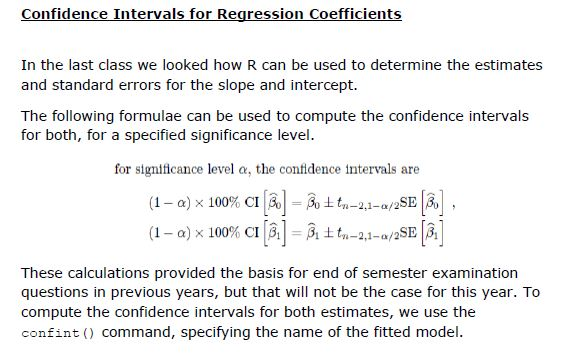
\includegraphics[width=1.1\linewidth]{images/RegressionConfInt}
	
\end{figure}
\begin{itemize}
\item You can be 95\% confident that the real, underlying value of the coefficient that you are estimating falls somewhere in that 95\% confidence interval. 
\item We can use confidence intervals as an alternative method of determining the outcome of hypothesis tests.

	\begin{description}
		\item[ $H_0$] $\beta_i = 0 $
		\item[ $H_1$] $\beta_i \neq 0$
	\end{description}

\item If the interval does not contain 0, we reject the null hypothesis. 
(this will coincide with the $p-$value being 0.05 or less.)
\item If the interval does contain 0, we fail to reject the null hypothesis. 
(this will coincide with the $p-$value greater than 0.05 )
\end{itemize}
\newpage

\subsection{Example 1}
Using the data from the previous example.
\begin{framed}
\begin{verbatim}
> confint(regr)
                     2.5 %     97.5 %
(Intercept)   -0.005867133 0.03515285
concentration  0.023448025 0.02572340
\end{verbatim}
\end{framed}
\begin{itemize}
	\item The 95\% confidence interval for the intercept estimate is $(-0.0058,0.0351)$.
	\item This confidence interval contains zero.
	\begin{description}
		\item[ $H_0$:] $\beta_0= 0 $ - FAIL TO REJECT NULL
		\item[ $H_1$:] $\beta_0 \neq 0$
	\end{description}
		\item The 95\% confidence interval for the intercept estimate is $(0.0234, 0.0257)$.
		\item This confidence interval does not contain zero.
		\begin{description}
			\item[ $H_0$:] $\beta_1= 0 $ - REJECT NULL
			\item[ $H_1$:] $\beta_1 \neq 0$
		\end{description}
\end{itemize}
\newpage
\subsection{Example 2}
\begin{figure}[h!]
\centering
\includegraphics[width=1.1\linewidth]{"images/RegressionConfInt - R Code"}
\end{figure}

\begin{itemize}
\item The intercept regression coefficient is 1.5178. The corresponding 95\% confidence interval is $(0.7597, 2.2760)$.
\item That confidence interval does not contain zero.
		\begin{description}
			\item[ $H_0$:] $\beta_0= 0 $ - REJECT NULL
			\item[ $H_1$:] $\beta_0 \neq 0$
		\end{description}
	\item The regression coefficient  for concentration is 1.9303. The corresponding 95\% confidence interval is $(1.8252,2.0354)$.
	\item Again that confidence interval does not containt zero.
	\begin{description}
		\item[ $H_0$:] $\beta_1= 0 $ - REJECT NULL
		\item[ $H_1$:] $\beta_1 \neq 0$
	\end{description}
\end{itemize}
\newpage
\end{document}